\section{物理過程のシミュレーション}

\begin{frame}[t,fragile]{物質中の中性子輸送}
  \begin{center}
  \resizebox{0.45\textwidth}{!}{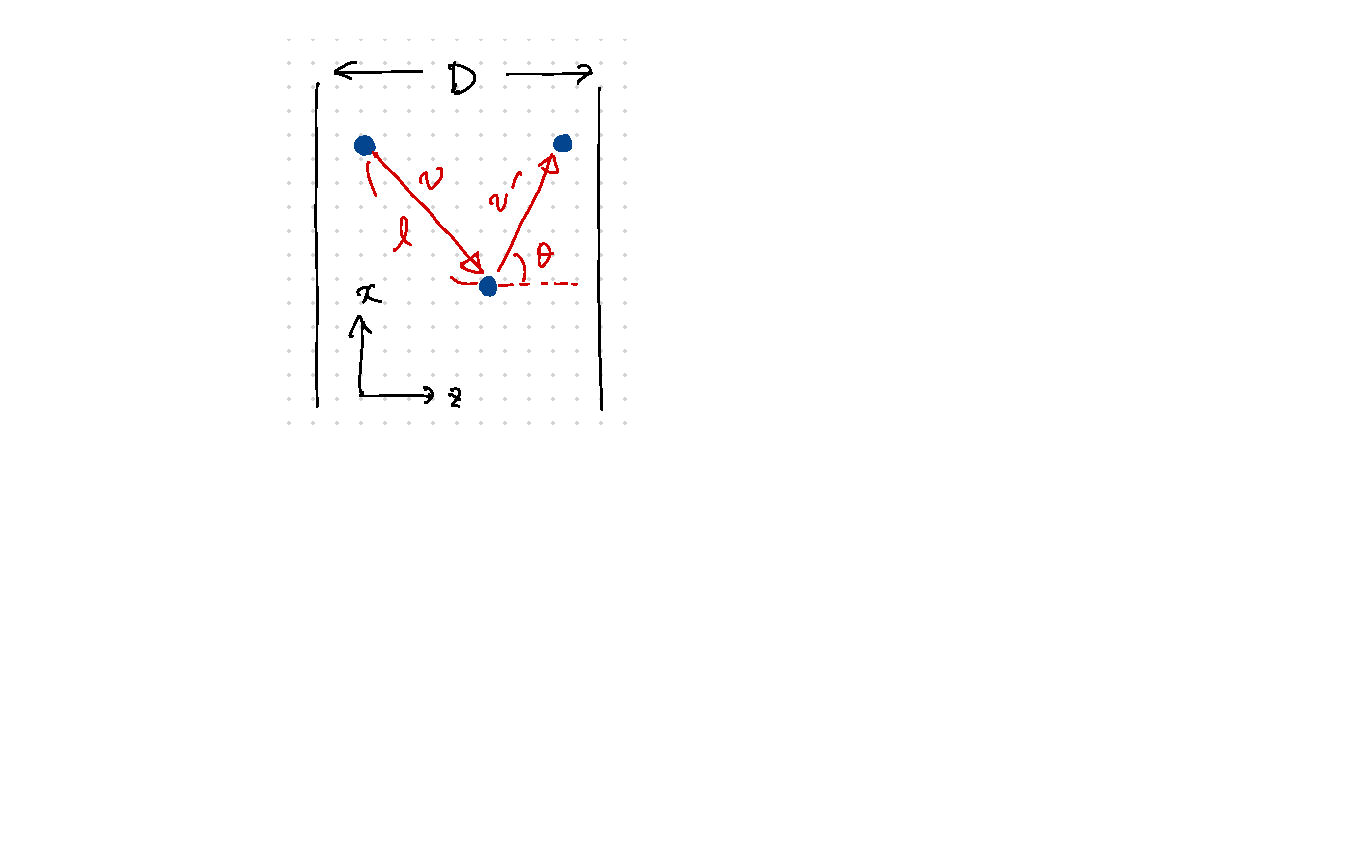
\includegraphics{image/scattering.pdf}}
  \end{center}
\end{frame}

\begin{frame}[t,fragile]{物質中の中性子輸送}
  \begin{itemize}
    %\setlength{\itemsep}{1em}
  \item ある板状の物質(厚さ$D$)に垂直に中性子が入射したときの吸収率・透過率・反射率
  \item 中性子はある確率で物質の原子核に衝突し、確率$p_{\rm c}$で吸収、$p_{\rm s}=1-p_{\rm c}$で散乱される
    \begin{itemize}
    \item 衝突は確率的に起きるので、次の衝突までの距離$\ell$は指数分布にしたがう($\ell$: 平均自由行程)
      \[
      p(\ell) = \lambda e^{-\lambda\ell}
      \]
    \item 衝突時、ランダムな方向に散乱されるとすると
      \[
      p(\theta,\phi) \, d\theta \, d\phi = \frac{d\Omega}{4\pi} = \frac{\sin \theta}{4\pi} \, d\theta \, d\phi
      \]
      \[
      p(\theta) = \frac{\sin \theta}{2} \qquad p(\phi)=\frac{1}{2\pi}
      \]
    \end{itemize}
  \end{itemize}
\end{frame}

\begin{frame}[t,fragile]{モンテカルロシミュレーション}
  \begin{enumerate}
    \setlength{\itemsep}{1em}
  \item 初期条件 $z=0$, $\theta = 0$
  \item {\color{red} 指数分布から$\ell$を選ぶ}
  \item $z \leftarrow z + \ell \cos \theta$
  \item $z<0$ → 反射(終了) \\
    $z>D$ → 透過(終了) \\
    $0 < z < D$ → 確率$p_{\rm c}$で吸収(終了)、$p_{\rm s}$で散乱
  \item {\color{red} 散乱後の$\theta$を選び}、2に戻る
  \end{enumerate}
  \vspace*{-5cm}\hspace{8cm}\resizebox{0.25\textwidth}{!}{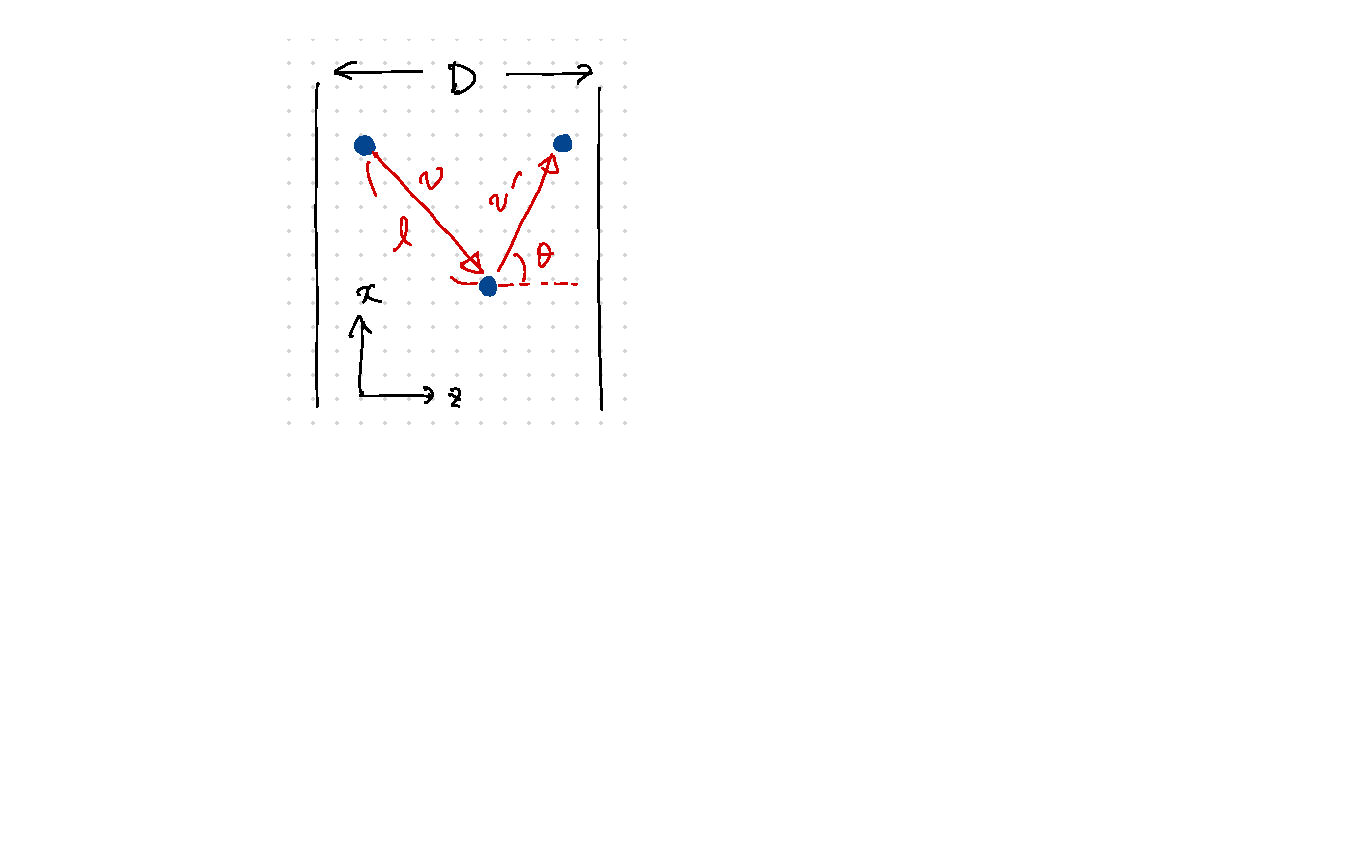
\includegraphics{image/scattering.pdf}}
\end{frame}

